% !TeX root = ../main.tex
% Add the above to each chapter to make compiling the PDF easier in some editors.

\chapter{Algorithms}\label{chapter:algo}
The minimax tree search algorithm is used to minimizing the possible loss for a worst case  scenario. It’s a recursive algorithm for choosing the next move in an two-player game. \newline A value is associated with each position or state of the game. This value is computed by means of a position evaluation function and it indicates how good it would be for a player to reach that position. The player then makes the move that maximizes the minimum value of the position resulting from the opponent's possible following moves. This can be extended if we can supply a heuristic evaluation function which gives values to non-final game states without considering all possible following complete sequences. We can then limit the minimax algorithm to look only at a certain number of moves ahead. In Reversi, the game often takes more than 60 turns to produce a winner, we use a heuristic function to evaluate the current game stage value by only looking ahead a couple of moves. This heuristic function is actually a collection of several heuristics and calculates the utility value of a board position by assigning different weights to those heuristics.
\section{Heuristics}
When looking at a Reversi board, its not clear at first sight which player has the advantage. Its easier to just focus on separated aspects of the playing board. Firstly we look at the coin parity, the most obvious one.
\subsection{Score Heuristic}
The \verb|int score_heuristic(board_t *board, disc_t player)| function returns the difference in coins between the max player and the min player.
\subsection{Mobility Heuristic}
The \verb|int board_mobility(board_t *board, disc_t player)| function attempts to capture the relative difference between the number of possible moves for the max and the min players, with the intent of restricting the opponent’s mobility and increasing one’s own mobility.\newline To compute the possible moves for a player, the paper “Bitboard Methodes for Games” \cite{quteprints85005} serves us with a fast function using bitwise operators. This function, which returns a bitboard, is called for both players. For the resulting bitboards the possible moves (bits set to 1) are counted. Finally the amount of possible moves the opponent has is subtracted from the possible moves the player has. 
\begin{lstlisting}[language=c]
size_t player_moves = bitboard_popcount(
  compute_moves(board->size, player_bitboard, opponent_bitboard));
size_t opponent_moves = bitboard_popcount(
  compute_moves(board->size, opponent_bitboard, player_bitboard));
return player_moves - opponent_moves;
\end{lstlisting}
\subsection{Stability Heuristic}\label{stable}
Since the aim is to have maximum discs at the end of the game, the number of your discs that are guaranteed to be there till the end is a good measure of the value of a position. Because these discs, called stable discs, cannot be flipped, they will stay till the very end and necessarily count towards your score. \newline The \verb|int board_stable(board_t *board, disc_t player)| function calculates  an estimated amount of stable discs a player has minus the estimated stable pieces the opponent has to offer. A key observation to make here is that discs placed on corner squares are always stable. Also, any disc on one of the edges of the board can only be flipped by a move along that edge. An edge disc therefore, is also stable if its next to a corner disc or another stable edge disc of the same color. Spinning this theory further, an algorithm came up to calculate the stable pieces.\newline For that algorithm, all 4 direction (north/south, west/east, nw/se, ne/sw) must be evaluated if a disc had either a border or a already stable disc is either of the two adjacent discs in that direction. Here is an example for the direction up/down.
\begin{lstlisting}[language=c]
candidates_up = player_bitboard >> shift_up;
candidates_up &=  ~(direction_1 & alread_stable_discs);
candidates_up = candidates_up >> shift down;
candidates_up ^= player;

candidates_down = player_bitboard >> shift_down;
candidates_down &= ~(candidates_down & alread_stable_discs);
candidates_down = candidates_down >> shift_up;
candidates_down ^= player;

stable_up_down = candidates_up | candidates_down;
\end{lstlisting}
\newpage
This proces needs to be repeated for all 4 directions. And in the end the stable disc bitboard can be updated.
\begin{lstlisting}[language=c]
alread_stable_discs |= 
  (stable_up_down & stable_west_east & stable_nw_se & stable_ne_sw);
\end{lstlisting}
This algorithm requires the board to remember its stable pieces for each player. This was done by adding two new bitboards to the board\_t struct. Annother sideeffect of this implmentation is, that it may need to be run several times to get all stable discs. Here the example for the black player.
\begin{lstlisting}[language=c]
bitboard_t check = board->stable_black + 1;
while(check != board->stable_black){
  check = board->stable_black;
  /* the void compute_stable_pieces(board_t *board, size_t size, 
   * bool is_black) function updated the bitboard board->stable_black */
  compute_stable_pieces(board, board->size, true);
}
\end{lstlisting}
It's important to notice, that this algorithm is only a negative estimation. It only calculates the stable pieces which are in direct or indirect contact to a corner square, but there are more discs, which can be stable. Stability occurs when a piece is in rows that are completely filled in all four flipping directions. It also occurs when a piece is next to a row of stable squares of its own color in each of the four directions \cite{ OthelloImplementation}. Here an example.
\begin{Verbatim}[frame=single]
   A B C D E F G H
1  O O X O _ _ _ _
2  O X O _ _ _ _ _
3  O ? O _ _ _ _ _
4  X O O _ _ _ _ _
5  O X _ _ _ _ _ _
6  _ X _ _ _ _ _ _
7  _ X _ _ _ _ _ _
8  O O _ _ _ _ _ _
\end{Verbatim}
Disc ? in b3 is a white disc and is stable, because in all four directions a row is either full or next to stable piece. But the algorithm above would not detect disc A as stable, hence the negative estimation which only returns a minimum of stable pieces.\newpage
\subsection{Disc Evaluation Heuristic}
A common practice in Reversi heuristics is, to give certain fields importance. For example there is the A-B-C-X method \cite{BrianRose}. The B-squares are in the center of the edge, the C-squares are on the edge next to the corner, and the A-squares lie between the B-squares and C squares. The X-squares are diagonally adjacent to the corners, with the ‘X’ indicating danger. Given the rules of the game, the only way for your opponent to take a corner is if you play in one of the squares next to a corner, i.e., the C-squares or X-squares. The X-squares are particularly dangerous, and a move to an X-square early in the game is almost certain to give up the adjacent corner. So we want moves, where the player places a disc on a “dangerous” square, to have a negative impact on the heuristic value. Therefor a grid with values for each square was created \cite{HeuristicEvaluation}.
\begin{center}
\begin{tikzpicture}
\draw[step=0.75cm,color=gray] (-3,-3) grid (3,3);
\matrix[matrix of nodes,nodes={inner sep=0pt,text width=.75cm,align=center,minimum height=.75cm}]{
	20 & -3 & 11 & 8 & 8 & 11 & -3 & 20 \\
	-3 & -7 & -4 & 1 & 1 & -4 & -7 & -3\\
	11 & -4 & 2 & 2 & 2 & 2 & -4 & 11\\
	8 & 1 & 2 & -3 & -3 & 2 & 1 & 8\\
	8 & 1 & 2 & -3 & -3 & 2 & 1 & 8 \\
	11 & -4 & 2 & 2 & 2 & 2 & -4 & 11\\
	-3 & -7 & -4 & 1 & 1 & -4 & -7 & -3\\
	20 & -3 & 11 & 8 & 8 & 11 & -3 & 20 \\};
\end{tikzpicture}
\end{center}
The \verb|int board_evaluat_discs(board_t *board, disc_t player)| function calculates the value of a current board, by adding the square values of the players positions and subtracting those of the opponent. Done is that trough bitboards. Here an example for the corner squares, each worth 20.
\begin{lstlisting}[language=c]
bitboard_t corners = 1;
corners = corners << 7;
corners += 1;
corners = corners << 49;
corners += 1;
corners = corners << 7;
corners += 1;
result += (bitboard_popcount(player_bitboard & corners) * 20);
result -= (bitboard_popcount(opponent_bitboard & corners) * 20);
\end{lstlisting}
This heuristic, contrary to all the other ones, only works on a 8x8 board.
\subsection{Frontier Heuristic}
In the Disc Evaluation Heuristic, we learnt about the value of X and B squares. In games between players that are both aware of the strategy, neither player will voluntarily make the sort of bad X-square and C-squares moves that give up corners for no reason. If you want your opponent to make these moves, then you will have to force him to do so. That is, you want to create a situation where the only moves available to your opponent are bad moves. \newline Frontier discs are defined as discs that border one or more empty squares. Although technically discs on the edge squares could fit this definition, they are not included when speaking of frontier discs. A move which creates many new frontier discs is called a loud move, while a quiet move creates relatively few frontier discs. A wall is a connected group of frontier discs of the same color. \newline Building a long wall leaves you with nothing to flip, cutting off your access to the squares on the other side of the wall. Meanwhile, the same wall gives your opponent a wide range of choices. Building walls and running out of moves usually go hand-in-hand.
In general, this means that quiet moves, which avoid creating a lot of frontier discs, are better than loud moves \cite{BrianRose}.\newline \newline The Algorithm checks for every disc, if it has an empty square in one of the eight directions (north, south, west, east, nw, ne, sw, se). Therefore, the player bitboard is shifted in one direction, ANDed with the empty squares and shifted back in the opposite direction(Opposite of north is south…).
\begin{lstlisting}[language=c]
bitboard_t empty = ~(player_bitboard | opponent_bitboard);
bitboard_t frontiers = 0;
bitboard_t matched;
for each direction d
	matched = empty & (player_bitboard >> shift_d);
	frontiers |= (matched >> shift_opposite_d);
\end{lstlisting}
In the Reversi game, A lot of frontier discs and walls will lower the probability of a player to win the game. So it would make sense to create a heuristic for walls as well, but this was not done in this implementation.\newline The \verb|int board_frontiers(board_t *board, disc_t player)| function returns:
\begin{lstlisting}[language=c]
-(my_frontiers - opponent_frontiers);
\end{lstlisting}
\newpage
\section{Weights}
The five different heuristics which are calculated for a specific board need to be weighted relative to their importance in the game. This is the crucial step for the Reversi AI. And also the hardest. It’s the hardest, because of several reasons.
\begin{enumerate}
	\item There is not a lot of research material. From reading through over 50 papers on Reversi AIs, only 2-3 gave an estimation of weights. On the other hand a lot of Reversi guides for human players tell the player on which objective he should focus in which stage of the game. In the AI it was a mixture of Brian Rose’s Othello a minute to learn.. A lifetime to master \cite{BrianRose}, and an Othello Program called Caesar build in 2003 by students \cite{Caesar}.
	\item In this implementation, the heuristics are not normed, which means, the return values for each heuristic have different maxima’s, minimums. For example the score heuristic returns a value between $-BoardSize^2$ and  $BoardSize^2$ and the disc evaluation heuristic a value between -360 and 360.
	\item To test the different weights an optimal case would be to have a better external Reversi AI to play against, which is still beatable and not deterministic. This way the current weights can play 100 games against the external AI and check how many games were won. After tweaking the weights the process is repeated until the maximum of wins is acquired. This was not possible in this case, because the three opponents to test the AI against (explained in Implementation \ref{subchapter:opponentAI}) served not as a good test opponent.
\end{enumerate}
Since the Caesar AI split the game up in 23 different stages and has a different weight for each of their 4 heuristic for every Stage as shown in this figure.\newline
\begin{center}
	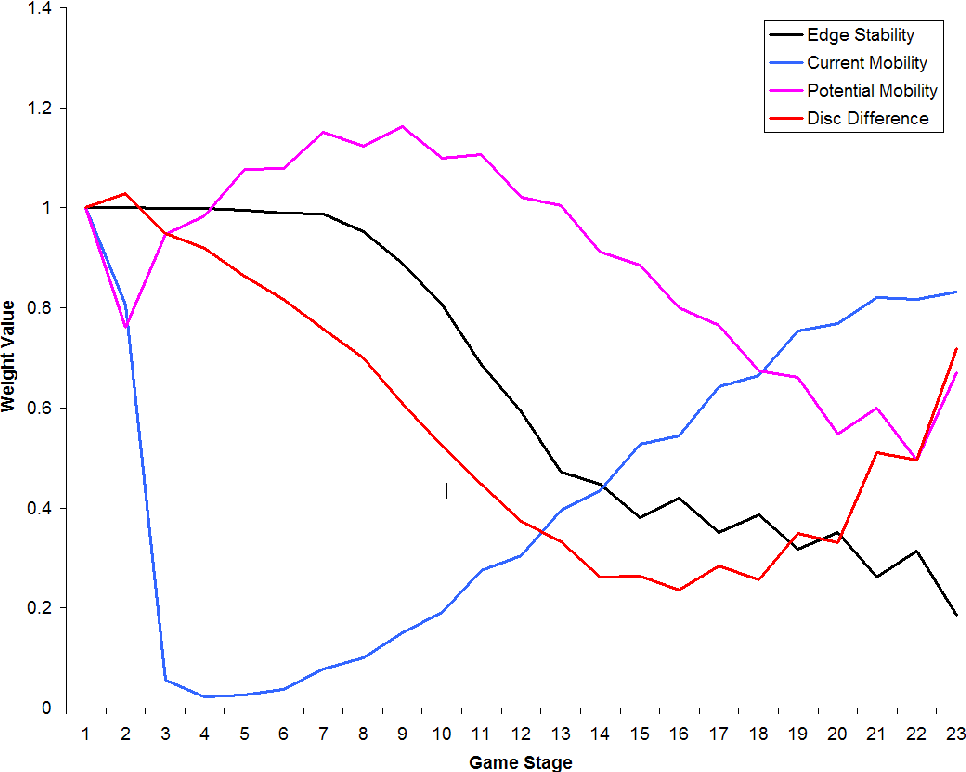
\includegraphics[width=10cm, height=7cm]{pictures/Ceasar}
\end{center}
This Reversi AI does a similar thing. The game is split up in 4 stages: Early game, Mid game, End game and End end game. Early game taking up the first third of the game, mid game the second third and end game the last third. End end game is only for the last 5 steps, because in those, certain heuristics such as disc evaluation or stability have less importance in comparison to score heuristic.\newline Here are the values for the different stages.
\begin{center}
	\begin{tabular}{ | m{3cm} | m{1.5cm}| m{1.5cm} | m{1.5cm}| m{3cm} | m{1.5cm} |} 
		\hline
		& Score & Mobility & Stability & Disc Evaluation & Frontier \\ 
		\hline
		Early Game & 1 & 8 & 20 & 7 & 3 \\ 
		\hline
		Mid Game & 3 & 2 & 10 & 4 & 3\\ 
		\hline
		End Game & 7 & 10 & 2 & 1 & 2\\ 
		\hline
		End end Game & 10 & 2 & 0 & 0 & 0\\ 
		\hline
	\end{tabular}
\end{center}
\section{End Game Search}
In the ending stages of a game, the branching factor gets bounded by the number of empty squares left on the board. As it turns out only a few of these are legal moves for either player - reducing the branching factor even further. Hence, it is possible to search much deeper in the end game than in the opening or the middle game. The goal was to make the Reversi AI a perfect end game player. The result is that it should plays a perfect game 9 suaqres from the end of the game. This was never really tested, it the game is perfect then, just assumed.\newline Done is that by counting the empty squares on the board, and if the are less or equal to 9, they are givin as the depth parameter to the minimax tree search function.

